\chapter{Migliorare la Generalizzazione}

La \textbf{Generalizzazione} rappresenta il cuore del Machine Learning: un modello non deve semplicemente memorizzare i dati del training set, ma dev’essere in grado di effettuare previsioni accurate anche su esempi mai visti prima. Per questo motivo, i dataset sono solitamente suddivisi in training set e test set: quest’ultimo non viene mostrato al modello durante l’addestramento, ma serve a valutare la capacità di generalizzazione. Nel Deep Learning, la questione diventa ancora più delicata: i modelli hanno un’elevata capacità espressiva e possono facilmente adattarsi in modo eccessivo ai dati di addestramento, fenomeno noto come \textbf{Overfitting}.

\section{Overfitting}

L’\textbf{Overfitting} si verifica quando un modello si adatta troppo ai dati di training, arrivando a modellare anche rumore e irregolarità accidentali, spesso dovute a errori di campionamento. In questi casi, il modello perde la capacità di distinguere tra regolarità significative e dettagli irrilevanti. Questo accade in particolare con modelli molto flessibili, che hanno una capacità sufficiente per apprendere qualsiasi cosa, incluse le fluttuazioni casuali dei dati.

\begin{quote}
\emph{"Se un modello è abbastanza potente da spiegare tutto, finirà per spiegare anche ciò che non è rilevante."}
\end{quote}

\begin{Osservazione}
    Visualizzare il fenomeno dell'overfitting, basta immaginare una persona che si veste con delle taglie di vestiti diverse, se un vestito risulta essere troppo aderente parleremo di overfitting, quando un vestito è troppo largo parleremo di underfitting.
\end{Osservazione}

\subsection{Prevenire l’Overfitting}

Per prevenire l’Overfitting, si possono adottare tre strategie principali, oltre a quelle già viste nel corso base di Machine Learning:

\begin{itemize}
    \item \textbf{Espandere il dataset}, ovvero ottenere più dati. È la soluzione più efficace, ma spesso difficile da realizzare nella pratica;
    \item \textbf{Utilizzare modelli con capacità adeguata}, evitando reti troppo semplici (Underfitting) o troppo complesse (Overfitting);
    \item \textbf{Combinare più modelli} (ensemble), utilizzando architetture diverse o addestramenti su sottoinsiemi dei dati.
\end{itemize}

L’espansione del dataset aiuta a ridurre il rumore e aumenta la significatività statistica. I modelli troppo complessi rischiano l’Overfitting, mentre quelli troppo semplici non riescono a catturare la struttura dei dati (Underfitting). Infine, l’ensembling permette di mediare tra i diversi comportamenti, bilanciando bias e varianza, questa possibilità viene effettuato utilizzando tecniche di \textit{Bagging} e di \textit{Boosting}, su cui ci soffermeremo più avanti.

\section{Limitare la capacità di un modello}

La capacità di un modello può essere controllata in diversi modi:

\begin{itemize}
    \item \textbf{Architettura:} definizione del numero di layer e neuroni;
    \item \textbf{Early Stopping:} interrompere l’addestramento prima che inizi l’Overfitting;
    \item \textbf{Weight Decay:} aggiungere una penalizzazione ai pesi grandi tramite regolarizzazione L1 o L2;
    \item \textbf{Noise Injection:} aggiungere rumore agli input o alle attivazioni per migliorare la robustezza;
    \item \textbf{Dropout:} È una delle forme di regolarizzazione più potenti e specifiche per il Deep Learning. Durante ogni passo dell'addestramento, una frazione casuale di neuroni viene temporaneamente "spenta" (le loro uscite vengono impostate a zero).
\end{itemize}

Tutte queste tecniche mirano a ridurre la complessità effettiva del modello, favorendo una maggiore capacità di generalizzazione,vediamole ora meglio.

\subsection{Early Stopping}

L’\textbf{Early Stopping} è una tecnica che interrompe l’addestramento nel momento in cui il modello inizia a sovra-adattarsi ai dati. Nelle prime fasi, i pesi sono piccoli e i neuroni operano nella regione lineare; col progredire dell’allenamento, i pesi aumentano, i neuroni entrano nella regione non lineare e il modello diventa più potente, rischiando però l’Overfitting. Fermare l’allenamento nel momento opportuno consente di mantenere una buona capacità predittiva. È pratica comune utilizzare un \textbf{Validation Set} per monitorare l’andamento dell’errore e decidere quando arrestare l’addestramento.

\subsection{Weight Decay}

La regolarizzazione L2 introduce un termine additivo nella funzione di costo per penalizzare i pesi grandi:

\begin{equation}
J(\theta) = \mathcal{L}(\theta) + \lambda \sum_i \theta_i^2
\end{equation}

Questo termine forza i pesi a rimanere piccoli, evitando soluzioni troppo complesse. Il parametro $\lambda$ controlla l’intensità della penalizzazione:

\begin{itemize}
\item $\lambda$ troppo grande $\Rightarrow$ Underfitting;
\item $\lambda$ troppo piccolo $\Rightarrow$ rischio di Overfitting.
\end{itemize}

La regolarizzazione L1 $ (\sum_i |\theta_i|)$ è un’alternativa che induce \textbf{sparsità}, cioè tende a portare molti pesi a zero, dunque adoperando una sorta di selezione delle features.

\subsection{Noise Injection}

Aggiungere rumore ai dati d’ingresso o ai pesi agisce come regolarizzatore. Ad esempio aggiungendo un \textbf{rumore Gaussiano}:
\[
x_t^{(noisy)} = x_t + \mathcal{N}(0, \sigma^2)
\]
Il rumore, amplificato dai pesi, penalizza indirettamente pesi grandi. L’effetto è simile al weight decay: il modello diventa più robusto e meno dipendente da feature specifiche.

\subsection{Dropout}

Il \textbf{Dropout} è una tecnica di regolarizzazione che disattiva casualmente neuroni durante l’addestramento. Ogni forward pass attiva una sottorete diversa, riducendo la dipendenza da co-attivazioni specifiche. Con \( H \) neuroni, si campionano \( 2^H \) reti. I pesi sono condivisi, quindi ogni sottorete è fortemente regolarizzata, il dropout permette di ridurre gli adattamenti complessi tra neuroni e rafforza la robustezza della rete.
\begin{figure}
    \centering
    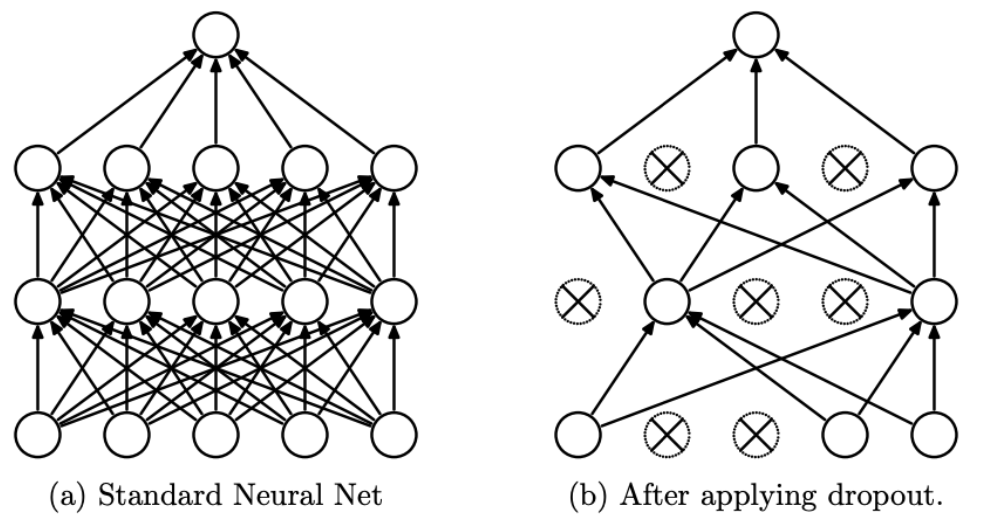
\includegraphics[width=0.85\textwidth]{figure/Dropout.png}
    \caption{Una Rete Neurale completamente connessa (a sinistra). La stessa Rete Neurale dopo che è stato applicato il Dropout (a destra).}
    \label{fig:dropout}
\end{figure}
Di conseguenza questa tecnica permette di avere due effetti principali:
\begin{enumerate}
    \item \textbf{Forza la robustezza:} I neuroni non possono fare affidamento sulla presenza di altri neuroni specifici e sono costretti a imparare feature utili e robuste in modo indipendente
    \item \textbf{Simula un ensemble:} Ad ogni iterazione, si addestra una "sottorete" diversa. Il risultato finale è un'approssimazione efficiente dell'addestramento e della media di un numero esponenziale di reti diverse che condividono i pesi.
\end{enumerate}

Pertanto il Dropout non è solo una forma di regolarizzazione numerica, ma impone una \textit{robustezza strutturale}, in cui ogni neurone dev’essere \textbf{indipendentemente utile}. Questo argomento può essere approfondito in Srivastava et al. 2014~\cite{srivastava2014dropout}.

\section{Ensembling}
Invece di cercare un singolo modello perfetto, le tecniche di ensemble combinano le previsioni di più modelli per ottenere un risultato più robusto e accurato. L'errore di un modello può essere scomposto in Bias (quanto le previsioni sono sistematicamente sbagliate) e Varianza (quanto le previsioni cambiano al variare del training set). L'ensemble è un modo potente per ridurre la varianza.

\[
\text{Errore totale} = \text{Bias}^2 + \text{Varianza} + \text{Rumore}
\]

Affinché un ensemble funzioni, i modelli che lo compongono devono essere diversi tra loro. La diversità può essere ottenuta addestrando modelli con architetture diverse, iperparametri diversi o su sottoinsiemi diversi dei dati. Le due strategie principali per creare ensemble sono:

\begin{itemize}
  \item \textbf{Bagging:} Si addestrano più modelli indipendentemente su diversi sottoinsiemi del training set, creati tramite campionamento con rimpiazzo. Le previsioni vengono poi aggregate (e.g media o voto di maggioranza). Il Bagging è particolarmente efficace nel ridurre la varianza di modelli complessi (basso bias, alta varianza);
  \item \textbf{Boosting:} Si addestrano modelli in sequenza. Ogni nuovo modello si concentra sugli errori commessi dai modelli precedenti, dando più peso agli esempi classificati erroneamente. Il Boosting è ottimo per ridurre il bias di modelli semplici (alto bias, bassa varianza).
\end{itemize}

\begin{figure}
    \centering
    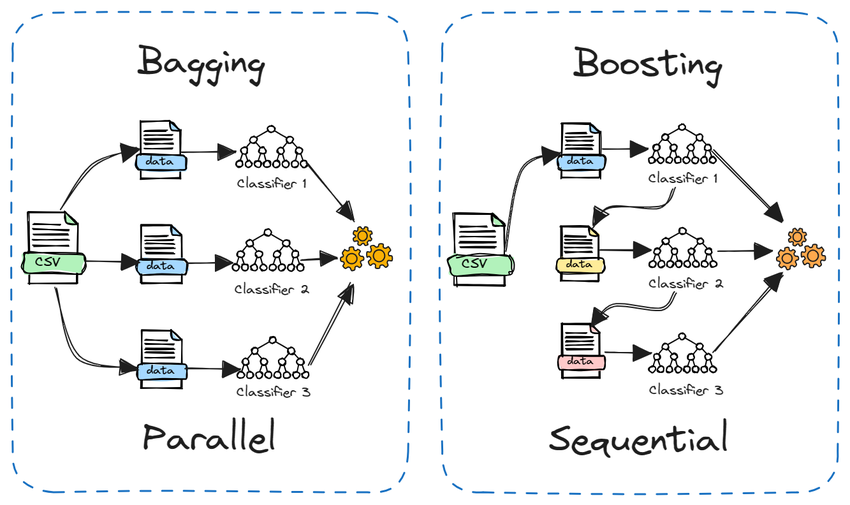
\includegraphics[width=0.6\textwidth]{figure/BagBoost.png}
    \caption{Rappresentazione dell’Ensemble tramite Bagging (modelli in parallelo) e Boosting (modelli in sequenza).}
    \label{fig:bagBoost}
\end{figure}

\section{Riepilogo delle Tecniche}
Non esiste una singola tecnica valida per ogni problema. Nella pratica, le strategie per migliorare la generalizzazione vengono spesso combinate. Ad esempio, è comune usare Data Augmentation, Weight Decay e Dropout contemporaneamente all'interno di una rete neurale. La scelta e la calibrazione di queste tecniche sono una parte fondamentale del processo di sviluppo di un modello di successo.

\begin{table}[h]
    \centering
    \caption{Strategie per migliorare la generalizzazione nei modelli di Deep Learning}
    \begin{adjustbox}{width=\textwidth}
    \begin{tabular}{@{}l|l@{}}
    \toprule
    \textbf{Tecnica} & \textbf{Descrizione} \\
    \midrule
    \textbf{Aumento dei dati} & Espandere il dataset con esempi reali o sintetici \\
    \textbf{Architettura adeguata} & Scegliere la capacità del modello con attenzione \\
    \textbf{Early Stopping} & Interrompere l’addestramento in tempo utile \\
    \textbf{Weight Decay} & Penalizzare pesi grandi nella funzione di loss \\
    \textbf{Noise Injection} & Aggiungere rumore a input o attivazioni \\
    \textbf{Ensemble} & Media di modelli diversi per ridurre la varianza \\
    \textbf{Bagging} & Campionamento con rimpiazzo per ensemble \\
    \textbf{Boosting} & Addestramento sequenziale di modelli deboli \\
    \textbf{Dropout} & Spegnere neuroni casualmente evitando adattamenti \\
    \bottomrule
    \end{tabular}
    \end{adjustbox}
\end{table}
